\chapter{問題提起と文献調査}
\label{related_works}

\section{問題提起}
人間が使用する道具に機械や情報処理が介在し、高度で複雑なシステムになった現在、人間と道具との関係が問い直され、その関係をいかに設計するか、すなわちヒューマンインターフェースデザインが必要となった。そして、原始的な道具の使用感と同じように、原因と結果の対応が直接的であり、その道具を使っているという意識がなくなる「道具の透明化」こそが、その理想であるとされてきた\cite{Watanabe2017}。インターフェース研究者の渡邊は、その理想を実現する指針として「自己帰属感」
\footnote{「自己帰属感」は、Gallagherの「ミニマルセルフ」における「Sense of Ownership」に対して渡邊が用いた訳語である\cite{Watanabe2017}。認知科学者・哲学者のGallagherは、自己を構成する2つの要素として、ミニマルセルフ(最小限の自己)とナラティヴ・セルフ(物語的自己)があると説明した\cite{Gallagher2000}。中でも「ミニマルセルフ」とは、一切の自己知識を失ったとしても残る最小限の自己であり、身体所有感(sense of ownership, body ownership)、行為主体感(sense of agency)の二つによって支えられていると説明する。こうしたGallagherの分類に基づき、それらを評価する方法が考案され、ラバーハンド錯覚実験などにみられるように、生来の肉体ではないものを自分の身体と錯覚してしまうような、人間の身体像の曖昧さに注目した研究が認知科学や心理学の領域で取り組まれてきた。}
という概念を導入し、例えばマウスカーソルやスマートフォンのような「操作時の指とグラフィックの追従性が高い」インターフェースは自身の一部や延長として感じられる、「透明」なインターフェースであると説明する。

確かにこうしたインターフェースを設計していくことは、複雑で高度な道具の力を借りて人間の活動の可能性を拡げることに貢献してきたが、人間と道具の関係とはそれだけだっただろうか?

渡邊の「自己帰属感」とは、使い手である「自己」がいて、その自己が思い通りに対象を使用できるよう、対象が自己に「帰属」する感覚についての説明である。しかし私たちの道具の使用とは、一方的に自分の意志を対象に入力し、具現化することだけに向いているのだろうか?その逆は考えられないのだろうか?

コンピュータ工学研究者のSydney Felsは、対象と人との関係性を、「Embodiment」の観点から4つに分類した\cite{Fels}。Embodimentとは日本語で「身体化、一体化、身体性」などと訳されるが、動詞の「embody」についてCambridge Dictionaryで引くと、"\textit{to include as part of something} ((何かを)何かの一部として取り込むこと)"とある\cite{embody}。ここで指摘したいのは、Embodimentの原義は「何かを取り込んで、何かの一部とすること」であり、「人がオブジェクトを取り込んで、一体化すること」のみを指すわけではないということだ。

しかし、Embodimentという言葉はHCIの分野でも用いられ、その文脈でのEmbodimentとは「使い手である人に、対象が取り込まれる」という意味でのEmbodimentである\cite{veq}。

FelsのEmbodimentにおいて特徴的なのは、「人が対象を取り込む」一体化だけでなく、「対象が人を取り込む」という逆向きの一体化についても論じていることである。この「対象が人を取り込む」という逆向きの関係性について、これまで注目されることは少なかったのではないだろうか。だが、(良さについて語る)。

一方的に使用するだけでなく、対象からの影響について折り合いをつけながら一体化していくような、いわば「人馬一体」のような一体感とはどのように生まれ、そしてそうした関係性が芽生える状況とはいかに設計できるのか。本研究では、こうした問いにアプローチしていくことを目指す。

% \section{Gallagherのミニマルセルフ}


% こうした研究で蓄積された実証的知見は、インターフェースデザインや身体拡張の設計・評価へと応用されている。インターフェース研究者の渡邊は、機械や情報処理が介在する高度で複雑な道具であっても、「使っている最中にはその道具自体を意識せずに身体の一部になったかのようになり、目的に集中できる」こと、すなわち「道具の透明化」という、ヒューマンインターフェースの理想を実現するための指針としてこの概念に注目する。渡邊は、例えばマウスカーソルやスマートフォンのような「操作時の指とグラフィックの追従性が高い」インターフェースには「自己帰属感(Gallagherのsense of ownershipに対する訳語)」が生じるとし、このことからこうしたインターフェースは「自身の一部、延長」として考えられ、「道具の透明化」が実現すると説明する\cite{Watanabe2013}\cite{Watanabe2017}。

\newpage

\section{FelsのEmbodiment}
Felsは、対象と人との関係性について、Reponse、Control、Gontemplation、Belongingの4つに分類した\cite{Fels}\cite{Costello2005}。それぞれの説明は以下の通りである(括弧内は筆者が訳語を当てた)。

\textbf{Response(応答):}\\
対象に対する働きかけの結果から、感情的な反応や理解を得る状態を指す。Felsはこの関係性の例として「コンピュータとそれに初めて触れた人」を挙げ、「なんらかの操作を通して得られた、便利な機能に喜んでいる状態、また逆に「有用な結果を得られず落胆する状態」と説明する。

\textbf{Control(制御):}\\
人が対象を自分自身の延長として使用し、その操作によって感情的な満足や美的体験を得る状態を指す。例えばピアノの演奏において、「音が出ている」ということだけでなく、自分自身の表現したいことが、不自由なくピアノを通して体現されていると感じるときの、一体感によってもたらされる心地よさがこれに該当する\footnote{「Control」においてFelsは、「自分自身の延長」として経験される感覚であり、またそれが追従性の高いグラフィックによってもたらされると説明する。これは、渡邊がマウスカーソルやスマートフォンに対して用いた「操作時の指とグラフィックの追従性が高い」インターフェースという説明と同等のものであると考えられる。このことからFelsのいうControlとは、Gallagherの「sense of ownership」と重なる。}。

\textbf{Contemplation(鑑賞):}\\
人が対象に対して働きかけることはないが、人がその対象からの信号やメッセージを内省や反映を通じて、感情的になったり美的体験を得る状態を指す。Felsはその具体例として、絵画の鑑賞体験を挙げる。

\textbf{Belonging(帰属):}\\
対象によって人が動かされているような経験を指す。人はその対象によって提供される体験を通じて感情的な反応を得る。ここでは、対象が人の体験や感情を形作る役割を果たす。たとえばバイクの運転において、「バイクに合わせた走り方をする」といったように、単にその対象を通して使い手の意図がそのまま体現されるのではなく、その対象に合わせた振る舞いがそこで形作られることに喜びを見出すような状態である。

\begin{figure}[H]
  \centering
  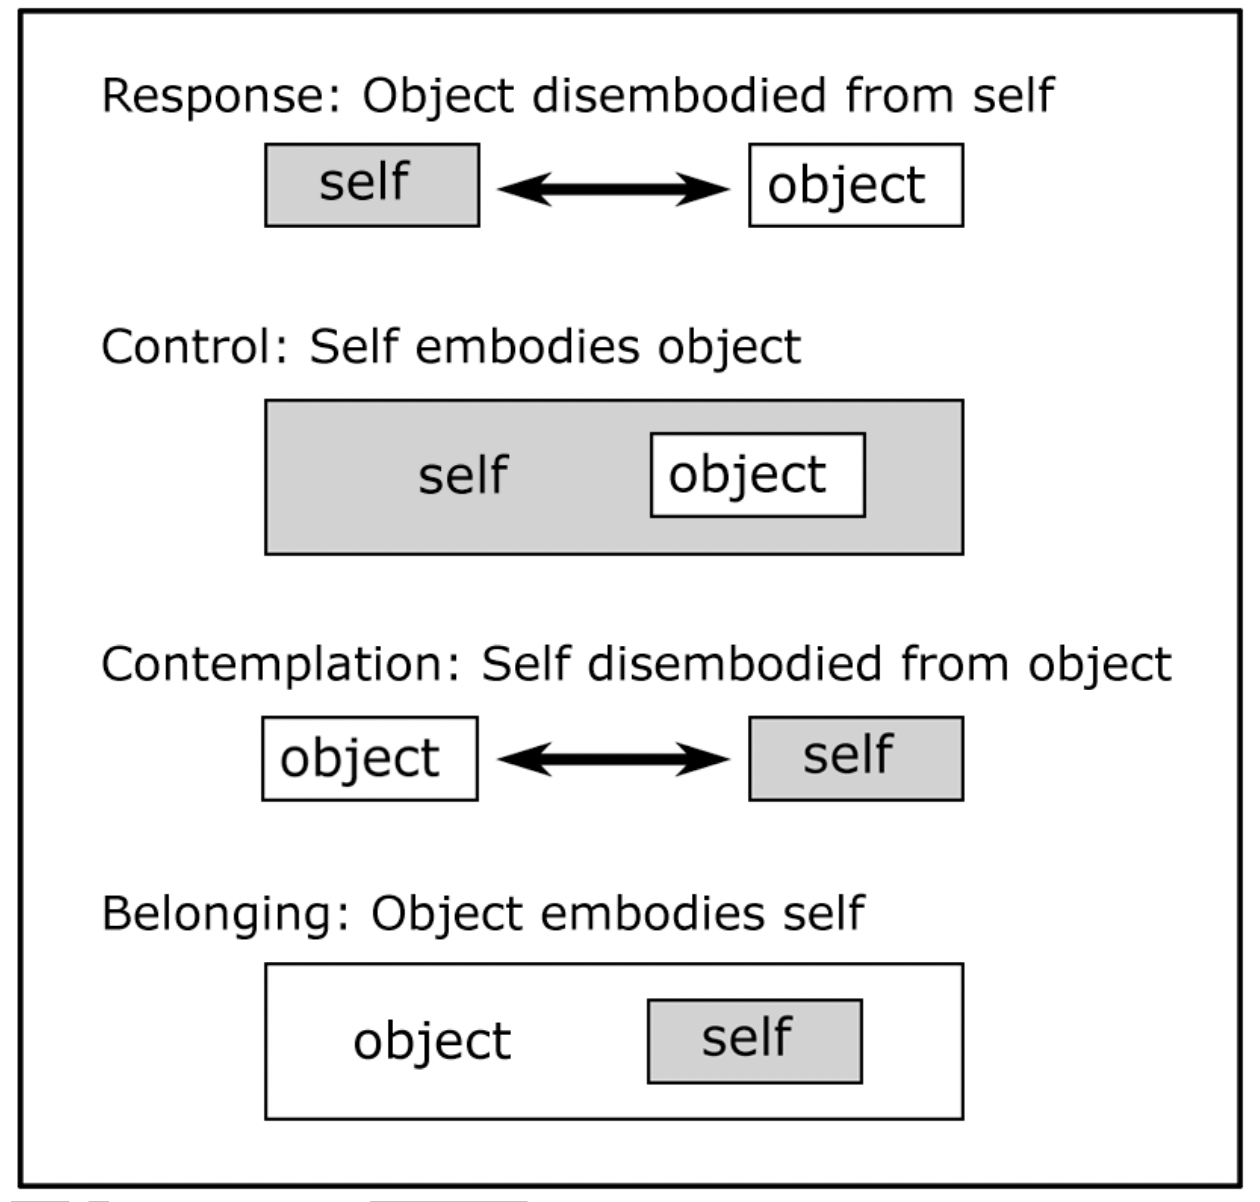
\includegraphics[width=8cm]{img/fels_diagram.png}
  \caption{FelsによるEmbodiment(仮置き)}
  \label{fig:fels_embodiment}
\end{figure}

% さて、Felsは特に、上記「制御 Control」においては「自分自身の延長」として経験される感覚について言及しており、またそれが追従性の高いグラフィックによってもたらされるという記述は、渡邊がマウスカーソルやスマートフォンに対して用いた「操作時の指とグラフィックの追従性が高い」インターフェースという説明と同等のものである。このことからFelsのいうControlとは、Gallagherの「sense of ownership」と同じものを指していると考えられる。その上で、Embodimentの状態をControlのみならずBelongingから捉えていること、そしてEmbodimentが生じていない状態についても言及していることなど、現在HCIの分野で一般に用いられる意味でのEmbodimentよりも広く、人と対象を捉えるモデルとなっていることが確認できる。

% さらにFelsは、対象と人とのあいだにある「深い関係」を指して、「Intimacy」という尺度で説明する。例えば楽器と人の関係性ように、Intimacyのある関係性のもとでは、「あたかもその装置が身体の延長であるかのように、考えや感情を効果的に表現できる」という。上記の、FelsによるEmbodimentの分類においては、ResponseがIntimacyの低い状態、ControlがIntimacyの高い状態として説明される。

冒頭で指摘した「逆向きの一体化」とは、Felsの分類におけるBelongingである。しかし、Belongingのような「逆向き」の影響を受けながら一体感を抱いている状態であっても、同時に人が対象に向けて「Control」することも同時に行われている。このように、自分の意志と道具の制約とのあいだで折り合いをつけることで得られる「親密な関係」を、Felsは「Intimacy」という言葉で説明した。

\section{リサーチクエスチョン}

これらの言葉を用いて本研究における問いを説明すると、次のようになる。

\begin{quote}
\textbf{対象からの影響も受けつつ(Belonging)、相互の折り合いをつけながら生まれる一体感(Intimacy)はどのように生まれ、そうした関係性が芽生える状況とはいかに設計できるのか。}
\end{quote}

そしてこの問いに応えるべく、手指の変換表現を通して探索的なリサーチを実施し、次章で説明する\textit{grasp}という概念に辿り着いた。そして、その概念をもとに上記の問いに答えられるような体験の設計を目指し、修士作品《Grasp(er)》を制作した。

\section{着想}
\label{prototyping_concept_making}
この問いは、「動きのスケッチツール」という目的で制作された習作「Digitalize」を展示した際の、体験者の様子を通して着想した。\\
静止画については「紙とペン」を通して直接イメージをスケッチできるが、動きについてはそれに相当するほど、直感的かつ、高い表現力でスケッチができるツールが見当たらなかった。そこで、動きに関して高い表現力を有する手指の動きを使って、「動きをスケッチする」ツールを設計することを案じていた。\\
しかし手指は人間の身体の中でもとりわけ随意に、高い表現力で動かすことのできる器官である。もし「手ではない形」を通してでも、様々な形や動きを自由に作れるのなら、人間の身体構造による制約を超えた「動きのスケッチ」ができるのではないか。そうして、手指の動きをトラッキングしつつ、画面上でその動きは別の形へマッピングされて動くインターフェースについて、プロトタイピングを行い、その過程をIAMAS Open House 2022にて展示した。この時点では、動きを記録する機能は存在しておらず、あくまで手と、それに伴って動く手指とは異なる形の動きが確認できるだけのものであった。

\begin{figure}[H]
  \centering
  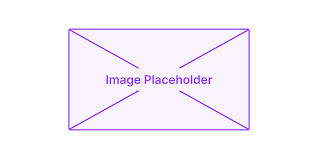
\includegraphics[width=15cm]{img/placeholder.png}
  \caption{IAMAS Open House 2022での展示のようす(2022年)}
  \label{fig:exhibit_2022}
\end{figure}

しかし実際に展示を行うとこの試作は、当初想定していなかった魅力があることに気づいた。それは、指の動きが単に、別の構造にマッピングされただけであるのに、別の構造の手を動かす体験はそれだけで興味を惹くものだということである。手指の変換が3パターン展示された状態のこの展示で、10分以上興味を持って体験する方が複数名いた。また、制作されたプロトタイプを展示した際、指先を動かすだけでなく、カメラに対して手を近づけたり遠ざけたり、手を裏返したりするなど、さまざまな体験の方法が現れた。

これは、「手指の動きに反応している」ということは分かっていても「どのように対応しているのか」についてははっきりせず、それを確かめるように身体を動かしていると考えた。

仕組みを知っている制作者はこうした試行をしないが、どのように変換されているのかを知り得ない体験者は、自身の体を動かして観察されたことでのみ、その動作原理を推測することになるので、最初にどう身体を動かしたかによって、動作原理をどう認識するかに違いが現れるのではないか。

この時のわかったようで分からない、行きつ戻りつな感覚に興味を持って体験し続ける様子に、「わかりやすさ」とは質の異なる楽しさがあると考え、そこに魅力を感じた。

\section{身体の変換や拡張を扱う先行事例(執筆中)}
身体の変換や拡張を行う研究は近年、数多く行われている\footnote{近年に多いとする根拠は、小鷹の「ラバーハンド錯覚の遅い発見問題」という問題意識に基づく。小鷹は、「ラバーハンド錯覚」というシンプルな錯覚が学術的にはじめて発表されたのが1998年と遅く、それが「コンピュータの普及により、事物を情報的に処理する感受性が世界に浸透しつつあった1990年代後半」であったことに、単なる偶然ではない「情報としての身体」という発想を後押しするものがあったのではないかと指摘する\cite{kodaka}。}\cite{Kondo2020, ekusute,Kasahara2017,augmented_hand_series}。
小川らによる「えくす手(Metamorphosis Hand)」\cite{ekusute}では、指の伸びた手などの現実の身体にはあり得ない特性を持ったバーチャルな身体を通じてピアノを演奏することができる。そのねらいは、「現実とは異なる特性のバーチャルハンドへの身体所有感の生起を通じ、現実の身体的制約を超えたインタラクションを実現する、一種のバーチャルな身体拡張体験を提供する」と説明される。

身体所有感の生起要因に関するこれまでの議論を参照し、本作は「テクスチャ、形状、空間的配置、解剖学的構造の4つの特性」を根拠に、身体所有感が生じながらも、自己身体と意味的に類似しないバーチャルハンドを制作している。これらの特性は、身体所有感を生じさせる上での実証的知見ではあるが、本研究が対象とするIntimacyは、例えば楽器のように、こうした生起要因を押さえなくとも、習得を経て生じうるのではないかと考える。また、生起要因を多く踏襲しているわけではないからこそ、身体所有感が生じるまでには期間を必要とし、その程度にも個人差が生じるのではないだろうか。これらの観点から、本研究の取り組みは「えくす手」よりも極端な身体変容を促す体験として位置付けられる。

佐藤雅彦らによる「君の身体を変換してみよ展」はさまざまなアプローチで身体の変容を扱う作品が展示されたが、その中でも「点にんげん・線にんげん」という作品は、ボディトラッキングを用いて取得された全身の関節の位置を捉えたキーポイントが点として扱われ、異なる方法で結びつけられたり、ボロノイ分割が適用される点群として扱われるなど、さまざまな「変換」が行われている。\\
本作品との構造上の相違点として、関節の位置を捉えたキーポイントの並び替えの有無が挙げられる。佐藤らの作品では、身体の関節の位置を捉えたキーポイントはその配置を変えることなく、繋げ方やインターフェースの文脈における位置付けの違いで展開される。一方、本作ではキーポイントの配列もダイナミックに変化する。これは、手指が複雑な動きのできる器官であると同時に、身体の中でもっとも随意に動かすことのできる器官でもあることから、構造が大きく異なる場合でも、手指の動きに連動している箇所を、動かしている中で容易に同定できると考えているためである。


